\documentclass[../../main.tex]{subfiles}

\begin{document}

\chapter{Theoretical Formulation} \label{chapter:theoreticalFormulation}

\section{Solution and constraint spaces} \label{section:solutionAndConstraintSpaces}

As stated in \S\ref{chapter:introduction}, the objective of this project is to find a way of sampling the space of viable solutions for a constraint, $V_c$.
Let $g'(l,c)$ be the learned generator function, as opposed to the true generator function.
Then let $V'_c$ be the learned viable space: the space of all solutions which can be obtained by passing a valid latent coordinate through $g'$:
\begin{equation}
	V'_c=\{s\;|\;g'^{-1}(s,c)\in L\}
\end{equation}
If $g$ is modelled by an artificial neural network then the condition that samples from $V_c$ can be drawn efficiently is satisfied when $g\approx g'\implies V_c\approx V'_c$, simply by sampling a point from $L$ and passing it through $g'$.

It is therefore necessary to define a distance metric for two spaces, which the neural network can be trained to minimise.
No single metric was found, however, which is both tractable and measures the distance between two general vector spaces.
The performance of the generator function will therefore be measured in two dimensions, each describing a desired trait of the learned viable space:
\begin{itemize}
    \item[] \textbf{Precision}: the proportion of samples from $g'$ which are actually members of $V_c$.
	\begin{equation}
		p(g')=\int_{C}\int_{L}\;1_{g'(l, c)\;\in\;V_c}\;\mathrm{d}l\;\mathrm{d}c
	\end{equation}
    \item[] \textbf{Recall}: the proportion of solutions which satisfy the constraint and are members of $V'_c$.
	\begin{equation}
		r(g')=\int_{C}\int_{V_c}1_{g'^{-1}(s,c)\;\in\;L}\;\mathrm{d}s\;\mathrm{d}c
	\end{equation}
\end{itemize}
Methods for estimating these quantities will be discussed in \S\ref{chapter:generatorTraining}.

Given that the network capacity is limited, a fundamental tradeoff exists between $p$ and $r$.
Too heavily weighting $p$ will result in a generator which picks from a small selection of promising solutions but misses many potential solutions; prioritising $r$ will result in a much larger range of solutions of which fewer satisfy the constraint.

This tradeoff is parameterised by a hyperparameter $w$ describing the weight of the $r$ in the loss function $\mathcal{L}$ that the neural network is trained to minimise.
The value of $w$ can be tuned to determine how confident the generator should be that its suggestions satisfy the constraint versus how confident it is that it is sampling from all viable solutions.
\begin{equation}
	\mathcal{L}(g')=p(g')+w\cdot r(g')
\end{equation}

\section{Modelling spaces as distributions} \label{section:modellingSpacesAsDistributions}

One limitation of using an ANN to model $g'$ is that $V'_c$ will always be unimodal (given that $L$ is unimodal), while $V_c$ will almost always be multimodal.
This arises as a consequence of the differentiability of ANNs, which is a desirable quality for this application so that gradient-based optimisation can be used in the latent space.
Therefore $p$ and $r$, as defined above, will carry very little meaning because almost all valid solutions will be in $V'_c$, even though small distances in the $L$ can be mapped to large distances in $S$ (effectively changing the frequency of solutions sampled from $g'$).

This problem is solved by modelling each space as a probability distribution and defining proxy measures for precision and recall.
The probability density of a distribution at a point is interpreted fuzzily as the likelihood that that point belongs to the space modelled by the distribution.
If the density at $a$ is greater than the density at point $b$, we say that $a$ is far more likely to belong to the space than $b$.
The probability distribution function (p.d.f.) representing a space $X$ is denoted $\hat{X}$.

Arbitrarily, $L$ is defined to be a uniform distribution within its bounds, which are set to 0 and 1 for the sake of simplicity.
\begin{equation}
	\hat{L}(l)=\left\{\begin{array}{ll}1&\mbox{if }0\le l_i\le1\;\forall\;\{i\;|\;1\le i\le k\}\\0&\mbox{otherwise}\end{array}\right.
\end{equation}
Since $V'_c$ is formed by passing $L$ through $g'$, its p.d.f. can be defined as the integral of $\hat{L}$ over all points in $L$ which map to that solution:
\begin{equation}
	\hat{V'_c}(s)=\int_{\{l\;|\;g'(l,c)=s\}}\hat{L}(l)\;\mathrm{d}l
\end{equation}
Finally, the true viable space's p.d.f. $\hat{V_c}$ is defined for any solution, and is $0$ if the solution does not satisfy the constraint, and $\gamma$ if it does.
The value of $\gamma$ is chosen such that the probabiliy mass of $\hat{V_c}$ is unity.
\begin{equation}
	\hat{V_c}(s)=\left\{\begin{array}{ll}\gamma&\mbox{if }h(c,s)=\text{satisfied}\\0&\mbox{otherwise}\end{array}\right.
\end{equation}
The continuity of ANNs should therefore not threaten the feasibility of this approach, because while regions of $S$ which are not part of $V_c$ may be sampled occasionally, if the generator is trained well then these regions will be much less probable than regions highly likely to satisfy the constraint (Figure \ref{fig:exampleMapping}).
Intuitively, this can be thought of as $g'$ pulling together the distinct modes of $V_c$, reducing the distance between them and thereby making it easier to find a global maximum by exploration.
\begin{figure}[H]
    \begin{center}
    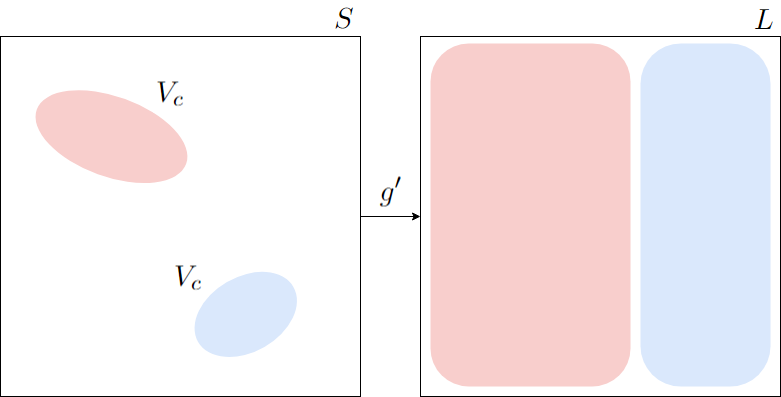
\includegraphics[width=0.75\textwidth]{exampleMapping}
    \caption{
		An example of how two distinct regions of $V_c$ in $S$ might be transformed by the generator to be much larger and closer together in $L$. 
    }
    \label{fig:exampleMapping}
    \end{center}
\end{figure}
Proxy metrics can now be defined which are intuitively similar to $p$ and $r$ but are functions of a p.d.f. rather than of $g'$ itself.
It is also possible to consider a distance metric between two distributions $-$ which is much easier to define than a distance metric between two spaces $-$ and minimise this directly, to prompt $\hat{V'_c}$ to match $\hat{V_c}$.
These avenues are explored in \S\ref{chapter:generatorTraining}.

\section{Adapting the GAN architecture} \label{section:adaptingTheGANArchitecture}

A probabilistic interpretation of vector spaces has been introduced which provides information on the density of points within the space, thereby working around the limitation of ANNs that prevents them discontinuous jumps between modes.
This will also later allow the definition of more tractable loss functions that can be used to train $g'$.
The network architecture, however, is still undefined.
\begin{figure}[H]
    \begin{center}
    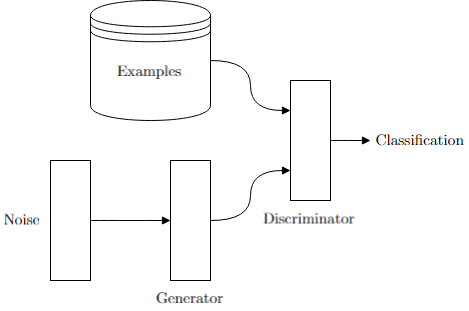
\includegraphics[width=0.65\textwidth]{ganArchitecture}
    \caption{
		A typical GAN architecture.
    }
    \label{fig:ganArchitecture}
    \end{center}
\end{figure}
GANs, introduced in \S\ref{section:adversarialAlgorithms}, are a family of ANNs which allow samples to be drawn from a distribution.
A typical GAN architecture has a generator, mapping samples from the latent space to the feature space, and a discriminator, which classifies feature vector as real or fake (Figure \ref{fig:ganArchitecture}).
This presents many similarities to the functions required to solve engineering problems, where the GAN's generator is similar to $g'$ and its discriminator models $h$.
As such, the GAN architecture was adapted slightly for this project.

\subsection{Pretrained discriminator} \label{subsection:pretrainedDiscriminator}

While training GANs, both the discriminator and generator are updated iteratively.
This forces the generator to learn a range of outputs $-$ effectively punishing low recall $-$ by having the discriminator adapt continuously to the changing output of the generator.

In an engineering problem, however, $h$ is fixed and does not change.
Whether $h$ is known in advance or learned from data, it does not make sense for it to be updated alongside the generator because of its immutability.
This has already been accounted for by defining loss as a combination of $p$ and $r$, forcing the generator to not overspecialise.

\subsection{Curried generator} \label{subsection:curriedGenerator}

Distributions learned by GANs are normally fixed.
The distribution $\hat{V_c}$ is parameterised by the constraint vector, however, and so any adapted GAN needs to be capable of taking a constraint as input and adapting its output accordingly.

Perhaps a more natural way of thinking about this is to consider $g$ as a curried function; that is, it takes a constraint and then returns another function which maps from the latent space to the solution space.
This is a subtle semantic difference to a dyadic function, but may provide direction as to the best way of integrating the constraint vector into the GAN.

Consider an ANN for multi-class classification \cite{ou07}.
When fed a feature vector, the activations of units in the hidden layers do not depend on the class; information about the class is only added in the output layer.
Likelihood estimates for each class are produced by multiplying the weight matrix of the final layer by the activations of the final hidden layer, and so are independent of each other.
The likelihood of each class can be viewed as the dot product of the final hidden layer's activations with a vector embedding of the class (\S\ref{section:representationLearning}).

$Q$-learning performed by Deep $Q$-Networks (DQNs) on a discrete action space work similarly \cite{mnih15}, except in a regression rather than a classification setting.
Crucially, the DQN is a function of two parameters (state and action) which has been curried to take only one parameter (state) with the other built into its weights; the $Q$-values produced for each action are independent of each other; the resulting $Q$-values represent an unbounded scalar instead of a probability, and; each $Q$-value is dependent only on the dot product of the final hidden layer's activations and a vector embedding of the related action.
So DQNs prove that it is possible to use ANNs as curried functions where the weights of the last layer only are varied as an embedding of the first parameter.

To adapt this to approximate $g'$, one needs only realise that a constraint embedding can be produced as a function of the constraint vector, which could feasibly be approximated by another ANN.
So information about $c$ can be passed into $g'$ by estimating the weights and biases of its output layer using two separate networks, the weight and bias embedders (Figure \ref{fig:curriedGenerator}), which takes only $c$ as input.
\begin{figure}[H]
    \begin{center}
    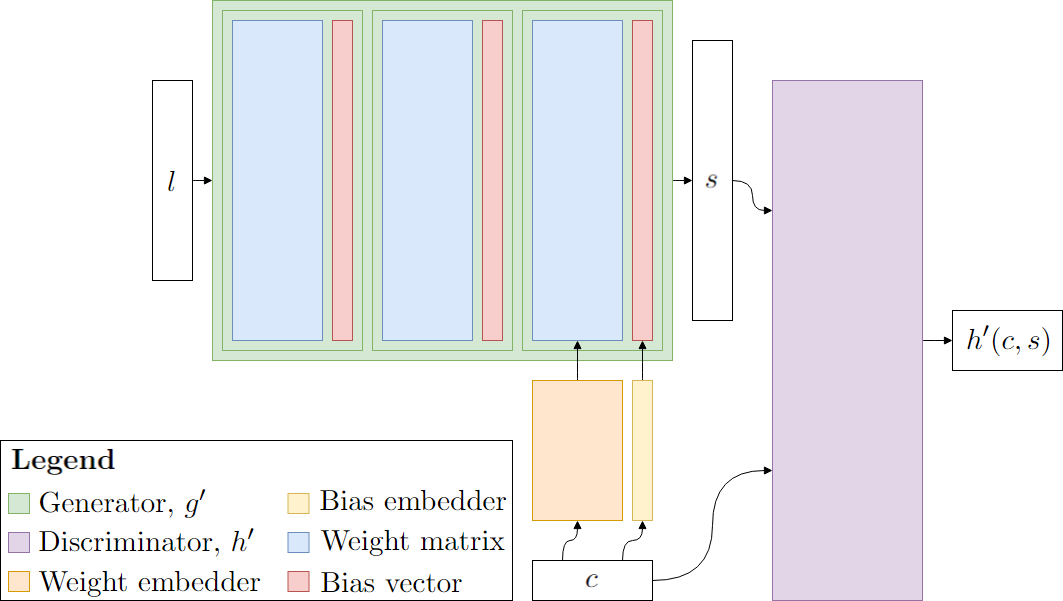
\includegraphics[width=0.8\textwidth]{curriedGenerator}
    \caption{
		Proposed architecture, with two networks estimating the weights and biases of the generator's output layer.
    }
    \label{fig:curriedGenerator}
    \end{center}
\end{figure}

\subsection{Data-free training} \label{subsection:dataFreeTraining}

If the discriminator has already been trained, or is known, no data are needed to train $g'$ because samples from $L$ can be used as training examples.
Hence, training data are only used as examples for training an approximation of $h$, $h'$, used as the discriminator; no additional data are needed to train $g'$.
The advantags to this approach are twofold: data are only needed to train $h'$ individually rather than adversarially in a GAN (which are notoriously hard to train \cite{bang18}), and $g'$ is only capable of overfitting to the extent that $h'$ has overfit its data.

When $h$ is known analytically, any overfitting of $g'$ can be combatted by increasing its capacity or training for longer.
When $h$ is modelled by a discriminator $h'$ learned from data, knowledge of the engineering environment can be used to augment data to alleviate overfitting (see \S\ref{chapter:discriminator}).
In any case, moving all responsibility for overfitting from $g'$ to $h'$ $-$ where it can be more easily measured and avoided $-$ is an exceptional advantage to adapting the GAN architecture in this way.

\end{document}
